\setauthor{Arwed Schnalzenberger}

\section{Einrichtung}
\subsection{Einrichtung des Azure Blob Storage}
\label{subsection:azure-blob-storage-getting-started}

Um die Effizienz bei häufigem Zugriff auf die Bilder möglichst effizient zu gestalten, 
wurden im Azure-Portal die folgenden Einstellungen konfiguriert.
\footnote{Infos dazu, was Azure Blob Storage ist und anderes stammen von hier: \cite{MicrosoftCorporationd}}

\subsubsection{SAS-Tokens}

Um den Zugriff auf Bilder über Shared Access Signatures (SAS) zu ermöglichen, muss in 
die Konfiguration ``Allow storage account key access'' aktiviert werden.

SAS-Tokens ermöglichen es uns, bestimmte Zugriffsrechte zu definieren, wie zum Beispiel
nur ein Lesezugriff. Das ermöglicht es unserem System, mittels Unity direkt auf die
gespeicherten Bilder zuzugreifen.

Mithilfe von SAS-Tokens die im Backend generiert und an Unity übergeben werden, 
kann Unity nun auf die benötigten Bilder zugreifen, ohne vollständige Zugriffsdaten 
des Storage Accounts zu benötigen. 

SAS-Tokens haben eine begrenzte Gültigkeitsdauer, was aus Sicherheitsgründen sinnvoll ist, 
da so der Zugriff auf Ressourcen zeitlich eingeschränkt wird. Das Backend übernimmt hierbei
die erneute Generierung dieser Tokens, sobald sie benötigt werden. Dadurch wird sichergestellt, 
dass autorisierte Nutzer:innen weiterhin auf die Ressourcen zugreifen können, ohne dass 
langfristig gültige Tokens ein Sicherheitsrisiko darstellen.
\footnote{Für Infos, wie Tokens generiert werden, siehe Kapitel \ref{subsection:sas-token-generation}}
\footnote{Alle Informationen zu SAS-Tokens stammen von: \cite{MicrosoftCorporationa}}


\subsubsection{Blob Access Tier}

Um den häufigen Zugriff auf Bilder effizienter zu gestalten, sollte in der Konfiguration 
des Blob Storage der Access Tier die Standardstufe auf ``Hot'' gesetzt werden.

Ein Azure Blob Storage bietet verschiedene Speicherstufen, wie ``Hot'', ``Cool'', ``Cold'',
oder ``Archive''. Cool ist zum Beispiel geeignet für weniger häufige Zugriffe, hat
niedrigere Speicherkosten, dafür aber höhere Zugriffskosten. 

Für uns ist Hot geeignet, da mit dieser Einstellung die Bilder für den häufigen 
Zugriff mit schnelleren Abrufzeiten optimiert werden und die Zugriffskosten niedriger sind. 
Dies führt allerdings zu höheren Speicherkosten. 
\footnote{Alle Informationen zu Blob Access Tiers stammen von \cite{MicrosoftCorporationb}}


\subsubsection{CORS-Header}

CORS (Cross-Origin Resource Sharing) ist eine Sicherheitsfunktion moderner Webbrowser, 
die den Zugriff auf Ressourcen zwischen verschiedenen Ursprüngen (Domains) einschränkt.
Da Memoryland und Unity Zugriff auf Bilder aus dem Azure Blob Storage benötigen, müssen
die folgenden CORS-Einstellungen für ``Blob-Services'' benötigt.

Es müssen die Spalten ``Allowed Origins'', ``Allowed Headers'' und ``Exposed Headers''
mit dem ``*'' Zeichen gefüllt werden, und Als ``Allowed Methods'', sollen ``Head'' und
``GET'' angegeben werden. Dies erlaubt den Zugriff von beliebigen Ursprüngen, mit beliebigen
Headern in der Anfrage. Weiters wird mit ``Exposed Headers'' eingestellt, dass alle 
Antwort-Header für den Client sichtbar sind und die ``Allowed Methods'' beschränkt die 
zulässigen HTTP-Methoden auf das Abrufen von Metadaten (HEAD) und das 
Laden von Bildern (GET). ``Max Age: 0'', verhindert das Caching der CORS-Vorgaben 
durch den Browser, sodass jede Anfrage die aktuellen Regeln berücksichtigt.

Wenn alles eingestellt wurde, können nun Bilder aus dem Blob Storage ohne Einschränkungen 
in Memoryland von überall auf der Welt angezeigt werden. 
\footnote{Alle Informationen zu CORS für Azure Blob Storage stammen von \cite{MicrosoftCorporationc}}


\subsection{Einrichtung von Azure PostgreSQL DB}

``Azure Database for PostgreSQL'' ist ein Datenbankdienst von Microsoft Azure, 
der auf dem Open-Source-Datenbanksystem PostgreSQL basiert 
\footnote{Weiter Infos zu Azure PostgreSQL: \cite{MicrosoftCorporationf}}. 
Er bietet eine Lösung für Anwendungen, die eine relationale Datenbank benötigen.

Die PostgreSQL Datenbank war eine schlüssige Entscheidung aufgrund der Erfahrung des Backend-Entwicklers.

\begin{table}[h t]
    \centering
    \caption{Vergleich: Flexible Server vs. Single Server}
    \label{tab:azure-postgresql}
    \begin{tabular}{lcc}
    \hline
    \textbf{Feature}                & \textbf{Single Server} & \textbf{Flexible Server} \\ \hline
    \textbf{Betriebssystem}         & Windows                & Linux                    \\
    \textbf{Maximale Speichergrö\ss{}e} & Bis zu 16 TB           & Bis zu 64 TB             \\
    \textbf{Hochverfügbarkeit}      & Nein                   & Ja (Zonenredundant)      \\
    \textbf{Kosten}                 & 1x                     & 2x (Compute + Storage)   \\ \hline
    \end{tabular}
\end{table}

Flexible Server haben gegenüber Single Server Unterschiede. 
Der wichtigste Grund für die Entscheidung war, dass Flexible Server auf Linux basiert, 
während Single Server Windows verwendet. 
\footnote{Warum Linux als Server-Betriebssystem verwendet wurde: \cite{hussain2015survey}}
\footnote{Alle Informationen zu ``Flexible Server vs. Single Server'': \cite{MicrosoftCorporatione}}

Au\ss{}erdem besitzen Flexible Servers eine grö\ss{}ere maximale Speichergrö\ss{}e, zonenredundante Hochverfügbarkeit, 
wodurch Ausfälle besser abgefangen werden können. Obwohl die Kosten etwas höher sein können, 
sind Flexible Servers aufgrund dieser Punkte die bessere Wahl für unser Projekt.

\subsection{Einrichtung von Azure AD B2C}

Die Einrichtung von Azure AD B2C wurde anhand des Beispiels im folgenden MSAL-Beispiel-Projekt
für Angular durchgeführt \cite{MicrosoftCorporationh}. Zusätzlich wurde die folgende
Website verwendet \cite{MicrosoftCorporationg}.
\footnote{Was ist \emph{Azure AD B2C} und warum verwenden wir es: Kapitel \ref{subsection:azure_ad_b2c}}

\subsection{Einrichtung von Azure WebApp}

Die Einrichtung der Azure WebApp wurde mithilfe der folgenden Website erledigt 
\cite{MicrosoftCorporationi}.
\footnote{Was ist \emph{Azure WebApp} und warum verwenden wir es: Kapitel \ref{subsection:azure_web_app}}


\subsection{Einrichtung von Azure Static WebApp}

Die Azure WebApp wurde nicht speziell konfiguriert, es gibt aber einige wichtige Aspekte, 
die vor dem Deployment der Angular Single Page Application beachtet werden müssen.  

Damit die Static WebApp die Routen korrekt erkennt und an die Single Page Application 
weiterleitet, anstatt ``\emph{404 Not Found}''-Fehler auszugeben, muss die folgende 
Konfiguration \ref{lst:staticwebapp-config} in der Datei ``\emph{staticwebapp.config.json}'' hinterlegt werden. 
Diese Datei muss sich im Verzeichnis des Angular-Projekts befinden -- in dieser Diplomarbeit
also im Ordner ``\emph{memoryland}''. \footnote{Infos zu dem Code \ref{lst:staticwebapp-config} gibt es in diesem Video: \cite{MicrosoftCorporationj}}
\footnote{Was ist \emph{Azure Static WebApp} und warum verwenden wir es: Kapitel \ref{subsection:azure_static_web_app}}

\begin{lstlisting}[numbers=left,caption={staticwebapp.config.json},label={lst:staticwebapp-config}]
{
    "navigationFallback": {
        "rewrite": "/",
        "exclude": [
            "*.{png,jpg,jpeg,gif,ico,css,scss,svg,js}"
        ]
    }
}
\end{lstlisting}


\subsection{Einrichtung des Backends}

Die Einrichtung des Backends für die Diplomarbeit erfordert die Konfiguration 
der ``\emph{appsettings.json}'' Datei. In dieser Datei stehen mehrere Einstellungen,
damit Memoryland auf die unterschiedlichen Dienste zugreifen kann. Die Konfiguration 
umfasst drei Hauptbereiche: Authentifizierung, Datenbank und den Azure Blob Storage.

\subsubsection{Authentifizierung}

Für die Authentifizierung wird Azure AD B2C genutzt, um die Benutzerverwaltung zu ermöglichen. 
In der ``\emph{appsettings.json}'' Datei sind die entsprechenden Einstellungen wie in dem folgendem
Beispiel (siehe Listing \ref{lst:appsettings-auth-config}) einzutragen. Hier werden unter anderem die Instance, ClientId und Domain des 
Azure AD B2C Verzeichnisses angegeben. Der SignedOutCallbackPath gibt den Pfad an, der nach 
der Abmeldung des:der Benutzers:in aufgerufen wird, und SignUpSignInPolicyId enthält 
den Namen der entsprechenden Policy. 
\footnote{Alle Informationen zu den Einstellungen der Authentifizierung sind hier zu finden: \cite{MicrosoftCorporationk}}

\begin{lstlisting}[numbers=left,caption={appsettings.json},label={lst:appsettings-auth-config}]
{
    "AzureAdB2C": {
        "Instance": "",
        "ClientId": "",
        "Domain": "",
        "SignedOutCallbackPath": "/signout/<SignUpSignInPolicyId>",
        "SignUpSignInPolicyId": ""
    }
}
\end{lstlisting}

\subsubsection{Datenbank}

Für die Konfiguration der Datenbank sind die entsprechenden Einstellungen, wie in dem folgendem
Beispiel (siehe Listing \ref{lst:appsettings-db-config}), ebenso in der Datei ``\emph{appsettings.json}'' 
einzutragen. Es gibt sowohl eine Einstellung für den Deployment-Datenbankanschluss (Default), 
als auch eine für den lokalen Anschluss (DefaultLocal), der für Test-Zwecke verwendet wird. 
Die UseLocalDb Einstellung gibt an, ob eine lokale Datenbank verwendet werden soll, wobei
\emph{false} bedeutet, dass die Deployment Datenbank verwendet werden soll.
\footnote{Alle Informationen zu den Einstellungen der Azure Datenbank sind hier zu finden: \cite{MicrosoftCorporationl}}

\begin{lstlisting}[numbers=left,caption={appsettings.json},label={lst:appsettings-db-config}]
{
    "UseLocalDb": false,
    "ConnectionStrings": {
        "Default": "",
        "DefaultLocal": ""
    }
}
\end{lstlisting}

\subsubsection{Azure Blob Storage}

Für die Konfiguration des Azure Blob Storage sind die entsprechenden Einstellungen, wie in 
dem folgendem Beispiel (siehe Listing \ref{lst:appsettings-blob-storage-config}), ebenso in der Datei 
``\emph{appsettings.json}'' einzutragen. Diese Einstellung ist notwendig, um die 
Anwendung mit dem Azure Blob Storage zu verbinden und den Zugriff auf Bilder und 
andere Dateien sicherzustellen.
\footnote{Alle Informationen zu den Einstellungen des Azure Blob Storage sind hier zu finden: \cite{MicrosoftCorporationm}}

\begin{lstlisting}[numbers=left,caption={appsettings.json},label={lst:appsettings-blob-storage-config}]
{
    "ConnectionStrings": {
        "BlobStorageDefault": "",
    }
}
\end{lstlisting}


\subsection{Einrichtung des Frontends}

Auch für das Frontend gibt es wichtige Einstellungen, damit die Single Page Application
funktioniert. Hierbei steht die Konfiguration in der Datei ``\emph{environment.ts}''.
Die Konfiguration ist für die Integration der Azure AD B2C Authentifizierung, sowie die 
Verbindung zum Backend und den APIs. Die Datei enthält alle wichtigen Daten für 
die Authentifizierung und die Verbindung zum Backend. 

Im Folgenden ist die Konfiguration beschrieben und in zwei Hauptkapitel unterteilt: 
\emph{environment.ts}-Konfiguration und Deployment.


\subsubsection{\emph{environment.ts}-Konfiguration}

Für die Authentifizierung wird Azure AD B2C verwendet. Die Konfiguration umfasst 
die folgende Definition (siehe Listing \ref{lst:environment-ts}) von Login- und Profil-Bearbeitungs-Flows.
\footnote{Die Informationen zu den Einstellungen stammen alle aus den folgenden Links: \cite{MicrosoftCorporationh} \cite{MicrosoftCorporationg}}

Userflows in Azure AD B2C sind vordefinierte, anpassbare Prozesse für häufige Benutzeraktionen 
wie Anmeldung, Registrierung, Profilbearbeitung oder Passwortzurücksetzung. Sie ermöglichen 
eine schnelle Konfiguration dieser Schritte, sodass Benutzer:innen nach Abschluss Zugriff auf 
die Anwendung erhalten.
\footnote{Die Informationen zu Userflows stammen alle aus dem folgenden Link: \cite{MicrosoftCorporationn}}

\begin{table}[h t]
  \centering
  \caption{Erklärung der Werte von ``\emph{environment.ts}''}
  \label{tab:environment-ts}
  \begin{tabular}{|l|l|}
  \hline
  \textbf{Wert}   & \textbf{Erklärung}                                                  \\ \hline
  signUpSignIn    & Der Name des Sign-Up/Sign-In Flows                                  \\ \hline
  editProfile     & Der Name des Profilbearbeitungs-Flows                               \\ \hline
  authority       & URL der Autorität, die für Authentifizierung genutzt wird           \\ \hline
  authorityDomain & Der Domainname des B2C-Tenants                                      \\ \hline
  clientId        & Die Client-ID der registrierten Anwendung                           \\ \hline
  redirectUri     & URI, wohin nach erfolgreicher Authentifizierung weitergeleitet wird \\ \hline
  scopes          & Liste von Berechtigungen, die die Anwendung benötigt                \\ \hline
  uri             & Die URI des Backend-Servers                                         \\ \hline
  \end{tabular}
\end{table}

\begin{lstlisting}[numbers=left,caption={environment.ts},label={lst:environment-ts}]
const b2cPolicies = {
  names: {
    signUpSignIn: "<flow-name>",
    editProfile: "<flow-name>"
  },
  authorities: {
    signUpSignIn: {
      authority: "https://<tenant-name>.b2clogin.com/
        <tenant-name>.onmicrosoft.com/<flow-name>"
    },
    editProfile: {
      authority: "https://<tenant-name>.b2clogin.com/
        <tenant-name>.onmicrosoft.com/<flow-name>"
    }
  },
  authorityDomain: "<tenant-name>.b2clogin.com"
};
    
export const environment = {
  production: false,
  b2cPolicies: b2cPolicies,
  msalConfig: {
    auth: {
      clientId: "<your-client-id>",
      authority: b2cPolicies.authorities.signUpSignIn.authority,
      knownAuthorities: [b2cPolicies.authorityDomain],
      redirectUri: '/',
    }
  },
  apiConfig: {
    scopes: [
      "https://<tenant-name>.onmicrosoft.com/<app-name>/<scope-name>",
    ],
    uri: "<backend-uri>"
  }
};    
\end{lstlisting}

Diese Konfiguration ermöglicht es, die Anwendung mit den Azure AD B2C 
Flows zu verbinden und eine sichere Kommunikation mit dem Backend sicherzustellen.

\subsubsection{Deployment}

All diese Einstellungen werden auch in GitHub (https://github.com/) benötigt.
Mithilfe von GitHub Actions \footnote{Alle Informationen zu GitHub stammen von hier: \cite{GitHuba}}
wird unser Frontend bei einem Push oder einer Pull-Request auf den Branch Main deployed.
Dafür müssen jedoch die folgenden Variablen \ref{tab:github-secrets} mittels GitHub Secrets im GitHub Repo eingetragen werden.
\footnote{Alle Informationen zu GitHub Secrets stammen von hier: \cite{GitHub}}

\begin{table}[h t]
    \centering
    \caption{GitHub Secrets für das Deployment des Frontends}
    \label{tab:github-secrets}
    \begin{tabular}{|l|l|}
    \hline
    \textbf{GitHub Secret}              & \textbf{Beschreibung} \\ \hline
    \texttt{B2C\_SIGNUP\_SIGNIN\_FLOW}   & Name des Sign-Up/Sign-In Flows \\ \hline
    \texttt{B2C\_EDIT\_PROFILE\_FLOW}    & Name des Profilbearbeitungs-Flows \\ \hline
    \texttt{B2C\_SIGNUP\_SIGNIN\_AUTHORITY} & Autoritäts-URL für den Sign-Up/Sign-In Flow \\ \hline
    \texttt{B2C\_EDIT\_PROFILE\_AUTHORITY}  & Autoritäts-URL für den Profilbearbeitungs-Flow \\ \hline
    \texttt{B2C\_AUTHORITY\_DOMAIN}      & Domain des B2C-Tenants \\ \hline
    \texttt{CLIENT\_ID}                  & Client-ID der registrierten Anwendung \\ \hline
    \texttt{SCOPE\_READ}                 & API-Berechtigung für Lesezugriff \\ \hline
    \texttt{SCOPE\_WRITE}                & API-Berechtigung für Schreibzugriff \\ \hline
    \texttt{BACKEND\_URI}                & URI des Backend-Servers \\ \hline
    \end{tabular}
    \caption{Verwendete GitHub Secrets für die Konfiguration}
\end{table}



\section{Technologien}
\subsection{.NET mit C\#}

C\# ist eine objektorientierte Programmiersprache, die speziell für die Entwicklung von 
Anwendungen auf der .NET-Plattform optimiert wurde. Als eine der fünf beliebtesten 
Programmiersprachen auf GitHub ist sie vollständig ``open-source''.

C\# greif die Konzepte aus JavaScript, Java und C++ auf, was sie für Leute mit Kenntnissen
in diesen Bereichen leichter zu lernen macht. Zu den zentralen Sprachmerkmalen gehören Generics, 
Pattern Matching, asynchrone Programmierung und Records. Diese Funktionen ermöglichen eine 
typsichere und strukturierte Entwicklung.

Für die Arbeit mit C\# stehen verschiedene Entwicklungsumgebungen und Werkzeuge zur Verfügung. 
Visual Studio bietet eine integrierte Entwicklungsumgebung mit umfangreichen Funktionen. 
Visual Studio Code stellt eine leichtgewichtige Alternative mit Erweiterungsmöglichkeiten 
dar. Zudem ermöglichen Kommandozeilen-Tools (CLI-Tools) eine flexible Nutzung. JetBrains Rider 
ist eine weitere IDE, die speziell für .NET optimiert wurde und in diesem Projekt genutzt 
wird. \ref{subsection:jetbrains-rider}

In dieser Diplomarbeit wurde C\# für das REST-Backend verwendet. Die zentrale Datenverwaltung 
erfolgte über Entity Framework Core mit einer PostgreSQL-Datenbank. Die Authentifizierung 
wurde durch die Anbindung an Azure AD B2C mittels MSAL realisiert. REST-APIs wurden implementiert, 
um die Kommunikation mit Unity und dem Frontend zu ermöglichen. Zusätzlich wurde Azure Blob 
Storage zur Speicherung und Verwaltung von Bilddateien integriert.

Die Wahl von C\# basiert auf zwei Faktoren. Die Sprache bietet eine direkte Integration mit 
Microsoft-Diensten, einschließlich der genutzten Azure-Dienste. Zudem wird C\# am meisten im 
Programmier-Zweig der HTL-Leonding unterrichtet, sodass bereits Vorkenntnisse vorhanden 
waren, die in der Diplomarbeit genutzt werden konnten.
\footnote{Alle Informationen zu C\# stammen von: \cite{MicrosoftCorporationo}}

\subsection{Entity Framework Core}

Entity Framework Core ist eine open-source Version des Entity Frameworks. Es dient 
als objektrelationaler Mapper (O\slash RM) für .NET-Anwendungen. Entity Framework Core ermöglicht 
die Arbeit mit relationalen Datenbanken unter Verwendung von .NET-Objekten und reduziert 
dabei den Aufwand für manuelle Datenzugriffslogik.

Der Datenzugriff erfolgt über ein Modell, das sich aus Entitätsklassen und einem 
Kontextobjekt zusammensetzt, welches bei uns ``ApplicationDbContext'' heißt. Dieses Kontextobjekt 
stellt eine Verbindung zur Datenbank her und verwaltet Datenbankabfragen sowie das Speichern 
von Daten. Entity Framework Core unterstützt verschiedene Ansätze zur Modellerstellung, 
darunter das Generieren eines Modells aus einer bestehenden Datenbank oder das manuelle 
Erstellen eines Modells, das anschließend mithilfe von Entity Framework Migrations in 
eine Datenbank überführt werden kann. In dieser Diplomarbeit wurde das Modell erstellt und dann
in eine Datenbank überführt.

Die Abfrage von Daten erfolgt über Language Integrated Query (LINQ). Änderungen an den Daten, 
wie das Erstellen, Modifizieren oder Löschen von Entitäten, werden über den DBContext 
vorgenommen und persistiert. Dabei stehen verschiedene Methoden zur Verfügung, 
um Daten effizient zu verwalten.
\footnote{Alle Informationen zu LINQ stammen von: \cite{MicrosoftCorporationq}}

Bei der Nutzung von Entity Framework Core sind verschiedene Aspekte zu beachten. Ein 
grundlegendes Verständnis relationaler Datenbanken ist erforderlich, um komplexe 
Datenbankoperationen effizient zu gestalten. Die Performance kann durch gezielte 
Optimierungen, wie den gezielten Einsatz von Indizes oder die Vermeidung von nicht 
skalierbaren Abfragen, verbessert werden.
\footnote{Alle Informationen zu Entity Framework Core stammen von: \cite{MicrosoftCorporationp}}


\subsection{MSAL}

MSAL (Microsoft Authentication Library) ermöglicht Entwickler das Abrufen von Sicherheitstoken 
von der Microsoft-Identity-Platform, um Benutzer:innen zu authentifizieren und auf gesicherte Web-APIs 
zuzugreifen. Sie kann verwendet werden, um sicheren Zugriff auf Microsoft Graph, andere 
Microsoft-APIs, Drittanbieter-Web-APIs oder eigene Web-APIs bereitzustellen. MSAL unterstützt 
viele verschiedene Anwendungsarchitekturen und Plattformen, darunter .NET, JavaScript, Java, 
Python, Android und iOS.

Für diese Diplomarbeit wurde MSAL verwendet, um eine benutzerdefinierte Authentifizierungslösung 
für das Angular-Frontend zu implementieren, die eine sichere Anmeldung und den Zugriff auf 
Web-APIs ermöglicht. Besonders hilfreich war MSAL bei der Anbindung an Azure AD B2C, da es 
eine einfache Handhabung der Authentifizierung und Tokenverwaltung ermöglichte.

Die Wahl von MSAL basiert auf der umfassenden Unterstützung durch Microsoft und der 
Integration in Azure-Dienste. Zudem wird MSAL in vielen verschiedenen Plattformen und 
Architekturen unterstützt, was es zu einer flexiblen Lösung für verschiedene Anwendungsfälle 
macht.
\footnote{Alle Informationen zu MSAL stammen von: \cite{MicrosoftCorporationr}}

\subsection{Postgres-DB}
\label{subsection:postgres_db}

PostgreSQL ist ein objektrelationales Open-Source-Datenbanksystem. Der Azure Database for 
PostgreSQL-Dienst von Microsoft bietet eine verwaltete Lösung, bei der Microsoft sich 
um Wartung, Sicherungen und Hochverfügbarkeit kümmert. Dies ermöglicht es Entwickler, 
sich auf die Entwicklung ihrer Anwendungen zu konzentrieren, anstatt sich um die 
Infrastruktur kümmern zu müssen. Besonders im Zusammenhang mit Cloud-Anwendungen 
bietet PostgreSQL in Azure Vorteile wie automatische Skalierbarkeit, hohe Verfügbarkeit 
und integrierte Sicherheitsfunktionen.

Für die Diplomarbeit wurde PostgreSQL aufgrund der Erfahrungen der oder die Entwickler gewählt. 
Die Nutzung von Azure Database for PostgreSQL erleichtert dabei die Verwaltung und 
bietet eine skalierbare Lösung, die den Anforderungen des Projekts gerecht wird.
\footnote{Alle Informationen zu MSAL stammen von: \cite{MicrosoftCorporations}}

\subsection{Cloud-Dienste mit Azure}

Azure bietet eine Vielzahl von Cloud-Diensten, die Entwickler Tools und Infrastruktur 
für ihre Anwendungen zur Verfügung stellen. Diese Dienste umfassen 
unter anderem unterschiedliche Speicherlösungen für unterschiedliche Arten an Daten, 
Identity-Management und Webhosting.
\footnote{Alle Basis-Informationen zu Azure stammen von: \cite{MicrosoftCorporationt}}

\subsubsection{Azure Blob Storage}
\label{subsection:azure_blob_storage}

Azure Blob Storage ist ein skalierbarer Speicherdienst. Er wird für unstrukturierte Daten, 
wie Bilder und Videos oder anderem, verwendet, wobei er das Speichern großer Datenmengen 
ermöglicht und eine kostengünstige Lösung für die Verwaltung und Sicherung von Dateien 
in der Cloud bietet. 

Die Wahl von Azure Blob Storage basiert auf der umfassenden Unterstützung durch Microsoft 
in .Net C\# und der hohen Verfügbarkeit und Sicherheit. Zudem ist es vorgesehen, dass in Memoryland
eine hohe Anzahl an Bildern gespeichert wird, wofür sich Azure Blob Storage eignet.
\footnote{Alle Informationen zu Azure Blob Storage stammen von: \cite{MicrosoftCorporationu}}

\subsubsection{Azure AD B2C}
\label{subsection:azure_ad_b2c}

Azure Active Directory B2C (Business to Consumer) ist ein Identity- und Zugriffsmanagement Dienst
Für diese Diplomarbeit wurde Azure AD B2C gewählt, um die Authentifizierung der Benutzer:innen
zentral zu verwalten. Da mit Azure AD B2C eine Integration mit anderen Azure Diensten, sowie mit
.Net besser von Microsoft unterstützt wird, war eine nahtlose Integration mit Azure AD B2C 
die optimale Lösung.
\footnote{Alle Informationen zu Azure AD B2C stammen von: \cite{MicrosoftCorporationw} \cite{MicrosoftCorporationx}}

\subsubsection{Azure WebApp}
\label{subsection:azure_web_app}

Azure App Service ist ein Dienst für das Hosting von Webanwendungen, REST-APIs und 
Backends. Er unterstützt verschiedene Programmiersprachen, darunter .NET, Java, 
Node.js, Python und PHP, und kann sowohl auf Windows- als auch auf Linux-basierten 
Umgebungen betrieben werden. Hierbei ist eine Azure WebApp eine spezifische Form
von Azure App Services.

Durch Funktionen wie automatische Skalierung, Lastverteilung und integrierte 
Sicherheitsmaßnahmen bietet Azure App Service eine stabile und zuverlässige 
Plattform für Webanwendungen.

Für diese Diplomarbeit wurde Azure App Service verwendet, um das Backend der 
Anwendung bereitzustellen. Der Dienst ermöglicht eine einfache Bereitstellung 
und Verwaltung der Web-API. Dank der automatischen Skalierung und Lastverteilung 
stellt Azure App Service sicher, dass die Anwendung auch bei höherer Nutzung 
performant bleibt.
\footnote{Alle Informationen zu Azure WebApp stammen von: \cite{MicrosoftCorporationy}}

\subsubsection{Azure Static WebApp}
\label{subsection:azure_static_web_app}

Azure Static Web Apps ist ein Cloud-Dienst zur Bereitstellung von Webanwendungen. 
Azure Static Web Apps deployt Code-Änderungen aus einem Repository automatisch. Der Dienst 
ist für Single-Page Applications (SPAs) optimiert und unterstützt Frameworks wie Angular, 
React, Vue, Svelte und Blazor.

Für diese Diplomarbeit wurde Azure Static Web Apps zur Bereitstellung des Frontens 
eingesetzt. Der Dienst ermöglicht eine nahtlose Integration mit GitHub, sodass Änderungen 
automatisch gebaut und veröffentlicht werden.
\footnote{Alle Informationen zu Azure Static WebApp stammen von: \cite{MicrosoftCorporationz}}

\subsection{JetBrains Rider}
\label{subsection:jetbrains-rider}

JetBrains Rider ist eine IDE (Integrated Development Environment) für die Entwicklung mit .Net. 
Rider unterstützt unterschiedliche .NET Framework-, Mono- und .NET Core-Projekte und bietet 
Unterstützung für Programmiersprachen wie C\#, VB.NET, F\#, ASP.NET, XAML, JavaScript, 
TypeScript, HTML, CSS, SQL und JSON.

Weiters besitzt Rider unterschiedliche Funktionen wie intelligenter Code-Vervollständigung, 
Refactoring-Werkzeuge und Debugging-Features, die bei der Entwicklung helfen. 

Für diese Diplomarbeit wurde JetBrains Rider als primäre Entwicklungsumgebung für die 
Backend-Entwicklung mit C\# und Entity Framework Core verwendet. Die IDE erleichtert 
die Arbeit mit .NET APIs und Datenbanken. Weiters wurde Rider aufgrund der 
Erfahrungen der Entwickler gewählt
\footnote{Alle Informationen zu JetBrains Rider stammen von: \cite{JetBrains}}

\subsection{CI/CD mit GitHub Actions}

GitHub Actions ist eine CI/CD-Plattform, die es ermöglicht, Build-, Test- und 
Deployment Prozesse direkt in einem GitHub-Repository zu automatisieren. Workflows 
werden in YAML-Dateien definiert und können bei bestimmten Ereignissen wie 
Code-Commits, Pull Requests oder Releases automatisch ausgeführt werden.

Für diese Diplomarbeit wurde GitHub Actions genutzt, um die automatische Bereitstellung 
der Anwendung sicherzustellen. Für diese Aufgabe wurde GitHub aufgrund der Erfahrungen
der Entwickler gewählt.
\footnote{Alle Informationen zu GitHub Actions stammen von: \cite{GitHuba}}


\subsection{Swagger \slash OpenAPI}

Swagger und OpenAPI sind Standards zur Beschreibung von REST-APIs. OpenAPI ermöglicht 
eine strukturierte Dokumentation von Endpunkten und deren Operationen, Parametern und
anderen. Weiters ermöglicht es noch einfache Authentifizierungsmethoden.

\begin{figure} [h t]
    \centering
    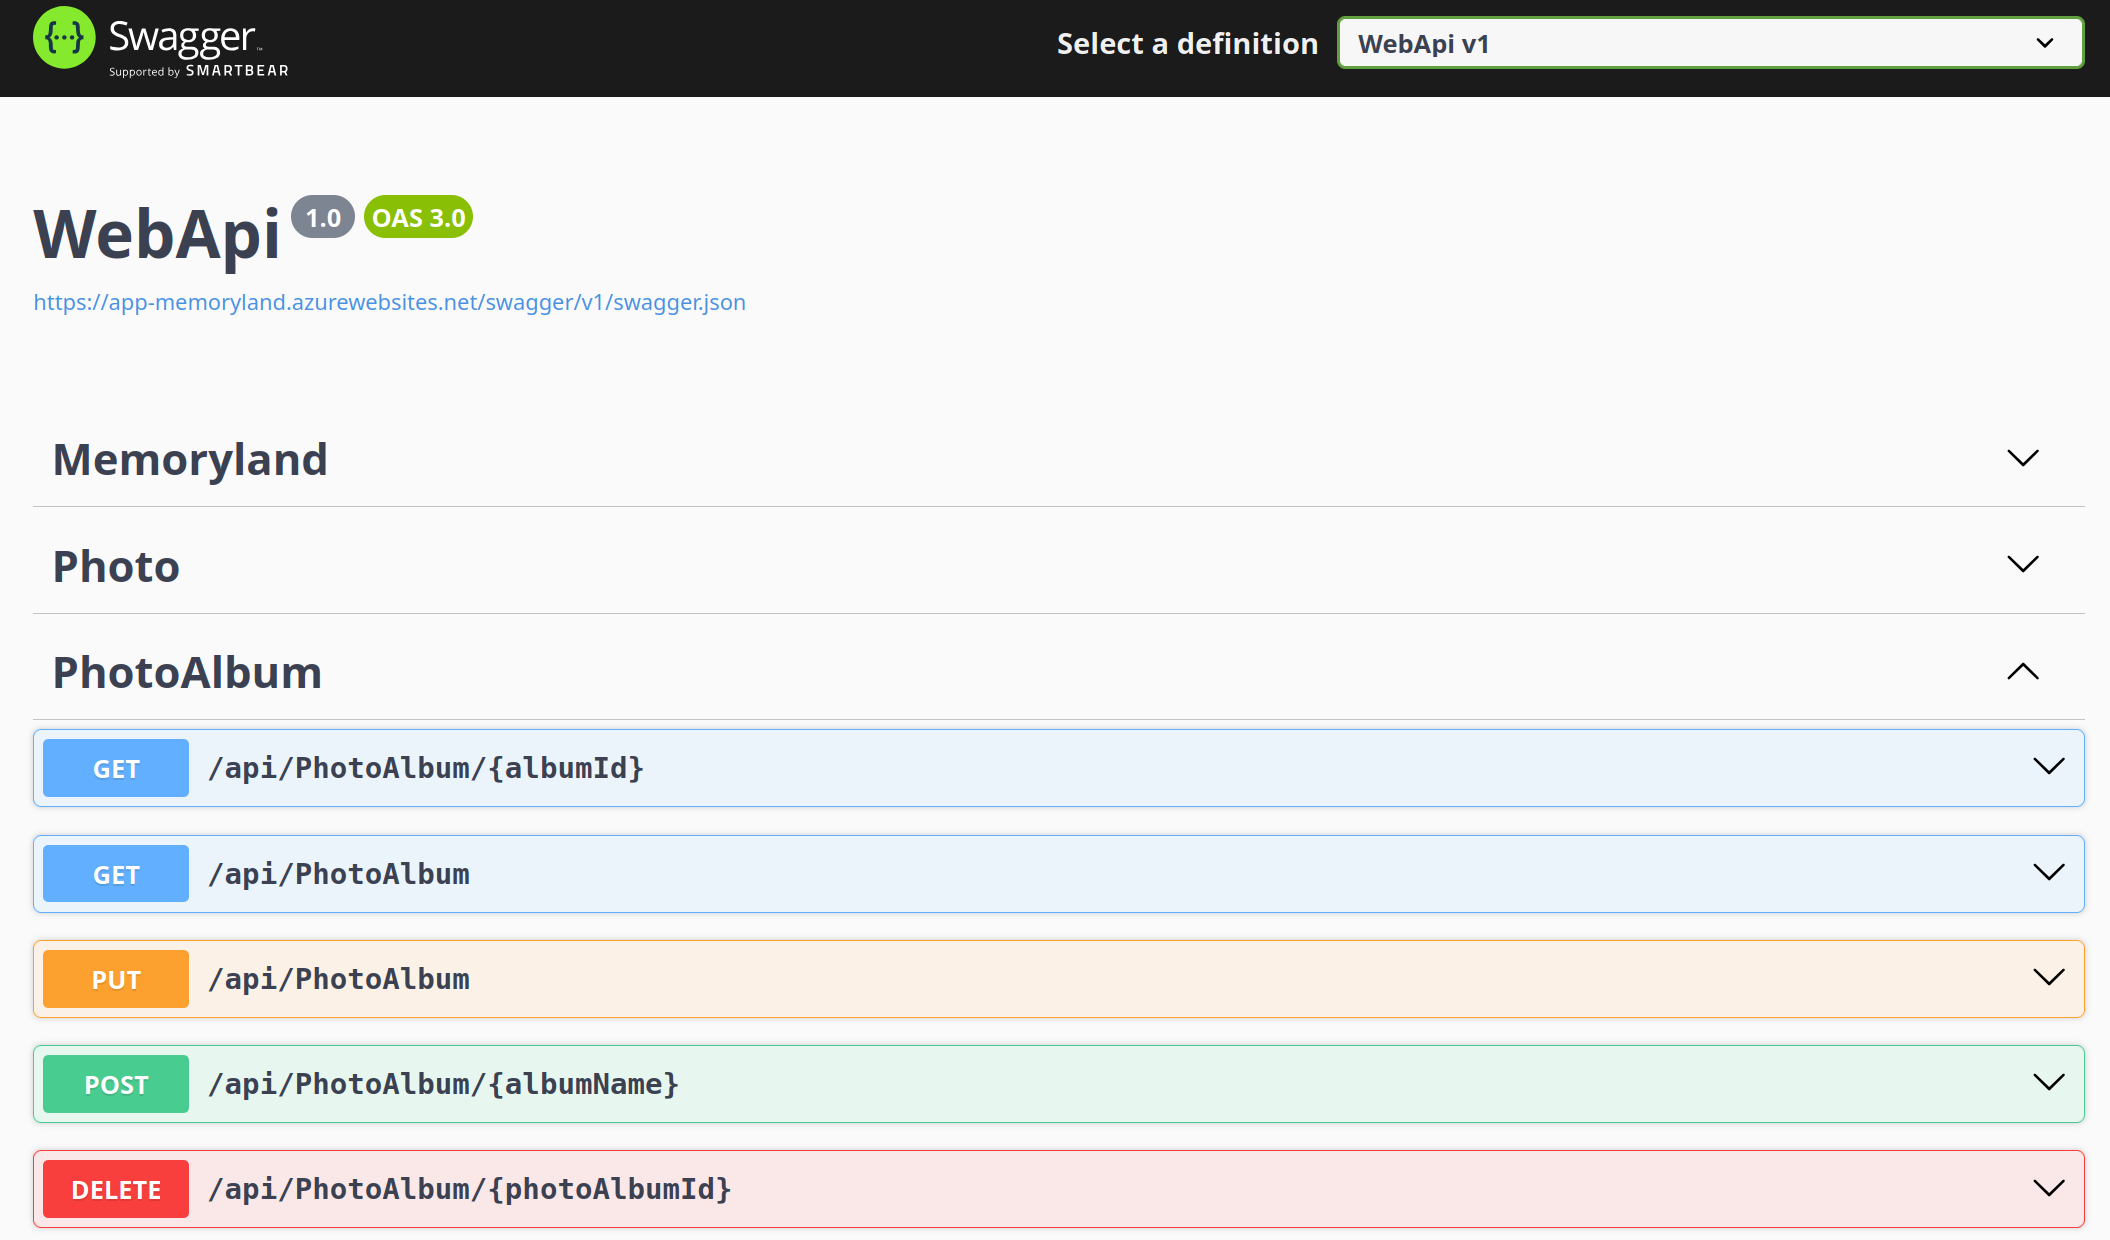
\includegraphics[scale=0.15]{pics/swagger-ui-example.png}
    \caption{Beispiel einer Swagger-UI}
    \label{fig:swagger-ui-example}
\end{figure}

Swagger beinhaltet eine Reihe von Tools, darunter die Swagger UI für interaktive 
API-Dokumentation und Swagger Codegen zur Generierung von Client-Bibliotheken.

Für diese Diplomarbeit wurde OpenAPI genutzt, um eine klare API-Dokumentation bereitzustellen. 
Die Swagger UI (User Interface) insbesondere erleichtert das Testen der API und erleichtert 
es das Frontend an das Backend zu verknüpfen.
\footnote{Alle Informationen zu Swagger und OpenAPI stammen von: \cite{SmartBearSoftware}}



\section{API}
In Memoryland wird eine Web-API eingesetzt, um die Verwaltung von Bildern, Alben
und anderen Daten im Backend zu steuern. Die API übernimmt dabei die Speicherung, 
Strukturierung und den Zugriff auf diese Daten, während das Frontend über die API 
mit dem Backend kommuniziert.

\subsection{Arbeiten mit C\#-Controllern}

Die API wurde mittels einer C\# WebAPI mit Controllern entwickelt. Diese auf dem .NET-Framework
basierende Technologie ermöglicht es uns RESTful-Endpunkte zu erstellen, über die das Frontend
mit dem Backend kommunizieren kann. Controller helfen uns dabei die unterschiedlichen Funktionen
des Backends in eigene Klassen zu unterteilen, was eine klarere Struktur ermöglicht.
\footnote{Alle Infos zu C\# WebAPIs mit Controllern stammen von: \cite{MicrosoftCorporationaa}}

Um Code-Verdoppelung zu vermeiden, wurde im Memoryland-Backend eine Basisklasse 
für API-Controller implementiert. Von der Klasse ``\emph{ApiControllerBase}'' \ref{lst:api-controller-base} 
erben alle anderen Controller, wodurch eine einheitliche Struktur sichergestellt und die Wartung 
erleichtert wird.

Die Base-Controller Klasse ist mit den zwei Attributen ``[ApiController]'' und 
``[Route(``api/[controller]'')]'' versehen. Mit dem ``[ApiController]''-Attribut 
erkennt das .Net-Framework die Klasse als API-Controller. Das 
``[Route(``api/[controller]'')]''-Attribut hingegen legt die Basisroute für alle Endpunkte 
der Controller fest, die von der ApiControllerBase erben. 
Der Platzhalter \emph{controller} wird durch den Namen des jeweiligen Controllers ersetzt. 
Beispielsweise erhält die UploadController-Klasse dadurch die Basisroute ``api/Upload''.

\begin{lstlisting}[numbers=left,caption={APIControllerBase.cs},label={lst:api-controller-base}]
using Microsoft.AspNetCore.Mvc;

namespace WebApi.Controllers;
    
[ApiController]
[Route("api/[controller]")]
public class ApiControllerBase : ControllerBase { }    
\end{lstlisting}

\subsubsection{Probleme bei der Implementierung}

Bei der Implementierung dieser Struktur kam es zu dem Problem, dass in ein paar Methodenrouten
ein führende Schrägstrich ``\slash'' verwendet wurde. Dies überschreibt jedoch die definierte
Basisroute des Controllers.

Beispielsweise führt die Angabe ``[HttpPost(``/picture'')]'' dazu, dass die Route nicht 
``api/Upload/picture'' lautet, sondern nur ``/picture''. Daher sollte in der Methodenroute 
kein führender Schrägstrich ``\slash'' verwendet werden.

Dies führte zu Problemen auch mit Swagger und OpenAPI, da diese Middleware versuchte, 
die Methode dem entsprechenden Controller zuzuordnen. Da der Controller eine Basisroute 
definiert hatte, jedoch die tatsächliche Route aufgrund des beschriebenen Problems nicht 
in diese Struktur eingebunden war, warf die Middleware den Error. Dies führte dazu, 
dass Swagger und OpenAPI die Methode nicht korrekt dokumentieren oder aufrufen konnten.

\subsection{Endpunkte in C\# Controllern}

Die Methode MyPostEndpointMethod \ref{lst:endpoint-example} stellt einen HTTP-POST-Endpunkt in einer Web-API bereit und
wird als Beispiel für die folgende Erklärung der Implementierung von Endpunkten in C\# Controllern
verwendet. Die Methode ist mit mehreren Attributen versehen, die Authentifizierung, 
Autorisierung und die API Route steuern. Das ``[Authorize]''-Attribut stellt sicher, 
dass nur authentifizierte Benutzer Zugriff auf die Methode erhalten, wobei es dafür
die in der Datei ``Program.cs'' definierte Technologie verwendet. Zusätzlich überprüft 
``[RequiredScope(``backend.write'')]'', ob der Benutzer über die notwendigen Berechtigungen 
verfügt. Diese Überprüfung basiert auf OAuth 2.0 und OpenID Connect und stellt sicher, 
dass nur Benutzer mit den nötigen Rechten (Scopes) bestimmte Operationen durchführen können. 

Mit dem ``[Route(...)]''-Attribut wird die Route der Methode definiert. Hierbei können in
geschwungenen Klammern ``\{ \}'' URL-Parameter definiert werden. Es können aber auch 
Objekte im Body des HTTP-Aufrufs mitgegeben werden. Dafür benötigt man das 
Attribut ``[FromBody]'' vor dem Parameter der Funktion setzen. Das JSON-Objekt wird dann
automatisch in die Objekt-Instanz deserialisiert und kann dann normal genutzt werden. 

Schlussendlich gibt die Methode dann ein Results-Objekt zurück, welches mehrere 
mögliche Antworttypen umfasst. Diese Antworttypen beinhalten die HTTP-Status-Werte.
Bei erfolgreicher Erstellung eines neuen Objekts wird also ein Created-Ergebnis zurückgegeben. 
Dies entspricht dem Status-Code 201. Falls die Anfrage fehlerhafte oder unvollständige Daten 
enthält, wird ein BadRequest<string> zurückgeliefert, welches auch zusätzliche Informationen
im ``string''-Format enthalten kann. Ist die Verarbeitung erfolgreich, aber kein neues Objekt 
erforderlich, wird stattdessen ein Ok<ReturnObj> zurückgegeben, welches wieder bestimmte
Typen enthalten kann, wie eine Liste an Bildern.
\footnote{Alle Informationen zur Implementierung von Endpunkten in C\# Controllern stammen von: \cite{MicrosoftCorporationaa} \cite{MicrosoftCorporationab}}

\begin{lstlisting}[numbers=left,caption={Beispiel eines Endpunkts},label={lst:endpoint-example}]
[HttpPost]
[Authorize]
[Route("mypath/{objId:long}")]
[RequiredScope("backend.write")]
public async Task<Results<Created, BadRequest<string>, Ok<ReturnObj>>> 
    MyPostEndpointMethod(
    long objId, 
    [FromBody] ObjDto postObjDto)
{
    ...
}
\end{lstlisting}

\subsection{API-Dokumentation mit Swagger und OpenApi}

Für eine übersichtlichere Dokumentation der API, wurde Swagger und OpenAPI eingesetzt.
OpenAPI ist eine Spezifikation zur Beschreibung und Dokumentationvon REST-APIs. Eine
OpenAPI-Datei enthält alle Informationen zu der API, einschließlich der verfügbaren 
Endpunkte, sowie der Ein- und Ausgaben. Diese JSON Spezifikation wird in diesem Projekt
automatisch erstellt.

Swagger ist eine Sammlung von Open-Source-Tools, die auf der OpenAPI Spezifikation 
aufbauen. Für diese Projekt wurde die Swagger UI verwendet, welches OpenAPI-Definitionen 
als interaktive Dokumentation darstellt, sodass API-Aufrufe direkt im Browser getestet 
werden können.
\footnote{Ein Beispiel einer Swagger-UI ist im Bild \ref{fig:swagger-ui-example} zu sehen.}

Durch den Einsatz von Swagger und OpenAPI wurde die Nutzung der API erleichtert, 
da die Entwickler die verfügbaren Endpunkte und deren Funktionalitäten direkt 
einsehen und testen konnten. 
\footnote{Alle Informationen zu Swagger und OpenAPI stammen von: \cite{SmartBearSoftware}}

\subsection{Erklärung der Controller und ihrer Aufgaben}

Die vier Controller in der API des Memoryland-Bakcends erfüllen jeweils spezifische 
Aufgaben im Zusammenhang mit der Verwaltung von Fotos, Alben, Uploads und deren Transaktionen.

\subsubsection{Album-Controller}

Der AlbumController ist zuständig für die Verwaltung von Fotoalben. Dieser Controller 
ermöglicht das Erstellen, Abrufen und Löschen von Alben, sowie das Zuweisen 
von Fotos zu Alben. \ref{tab:album-controller}

\begin{table}[h t]
    \centering
    \caption{Album Controller Endpunkte}
    \label{tab:album-controller}
    \begin{tabular}{|l|p{5cm}|l|p{5cm}|}
    \hline
    \textbf{Methode} & \textbf{Pfad} & \textbf{Authorized} & \textbf{Beschreibung} \\ \hline
    GET & /api/PhotoAlbum\break{/\{albumId\}} & Ja & Ruft ein Fotoalbum mit der angegebenen ID ab. \\ \hline
    GET & /api/PhotoAlbum & Ja & Ruft eine Liste aller Fotoalben ab. \\ \hline
    PUT & /api/PhotoAlbum & Ja & Bearbeitet den Namen eines Fotoalbums. \\ \hline
    POST & /api/PhotoAlbum\break{/\{albumName\}} & Ja & Erstellt ein neues Fotoalbum mit dem angegebenen Namen. \\ \hline
    DELETE & /api/PhotoAlbum\break{/\{photoAlbumId\}} & Ja & Löscht ein Fotoalbum mit der angegebenen ID. \\ \hline
    \end{tabular}
\end{table}


\subsubsection{Memoryland-Controller}

Der MemorylandController ist für die Verwaltung und Interaktion mit Memorylands 
verantwortlich. Dabei werden Memorylands, die Positionierung der Bilder in Memorylands
und Tokens für den Zugriff auf Memorylands verwaltet. \ref{tab:memoryland-controller}

Konfigurationen von Memorylands sind hier beschrieben \ref{sec:memoryland-config}.

\begin{table}[h t]
    \centering
    \caption{Memoryland Controller Endpunkte}
    \label{tab:memoryland-controller}
    \begin{tabular}{|l|p{5cm}|l|p{5cm}|}
    \hline
    \textbf{Methode} & \textbf{Pfad} & \textbf{Authorized} & \textbf{Beschreibung} \\ \hline
    GET & /api/Memoryland/all & Ja & Gibt eine Liste aller Memorylands zurück. \\ \hline
    GET & /api/Memoryland & Nein & Gibt eine Memoryland mit all dessen Bildern zurück. Dafür wird ein Token benötigt \\ \hline
    PUT & /api/Memoryland & Ja & Bearbeitet den Namen eines Memorylands. \\ \hline
    GET & /api/Memoryland/\{id\}\break/configuration & Ja & Gibt die Konfiguration für das angegebene Memoryland zurück. \\ \hline
    GET & /api/Memoryland/types & Nein & Gibt die verfügbaren Typen für Memorylands zurück. \\ \hline
    GET & /api/Memoryland/\{id\}\break/token & Ja & Gibt das Token für das angegebene Memoryland zurück. \\ \hline
    POST & /api/Memoryland/\{id\}\break/token & Ja & Erstellt ein neues Token für das angegebene Memoryland. \\ \hline
    POST & /api/Memoryland\break/\{memorylandName\}\break/{memorylandTypeId} & Ja & Erstellt ein Memoryland mit dem angegebenen Namen und Typ. \\ \hline
    POST & /api/Memoryland\break/\{memorylandId\} & Ja & Erstellt eine Konfiguration für das Memoryland. \\ \hline
    DELETE & /api/Memoryland\break/\{memorylandId\} & Ja & Löscht das angegebene Memoryland. \\ \hline
    DELETE & /api/Memoryland/config\break/\{id\} & Ja & Löscht die angegebene Konfiguration eines Memorylands. \\ \hline
    \end{tabular}
\end{table}


\subsubsection{Foto-Controller}

Der FotoController ist für die Verwaltung von Fotos verantwortlich. Dies umfasst das 
Abrufen, Erstellen und Löschen von Fotos, sowie das Verwalten der Fotodaten, die in 
Alben gespeichert sind. \ref{tab:foto-controller}

\begin{table}[h t]
    \centering
    \caption{Foto Controller Endpunkte}
    \label{tab:foto-controller}
    \begin{tabular}{|l|p{5cm}|l|p{5cm}|}
    \hline
    \textbf{Methode} & \textbf{Pfad} & \textbf{Authorized} & \textbf{Beschreibung} \\ \hline
    GET & /api/Photo/\{albumId\}\break/\{photoName\} & Ja & Ruft ein Foto aus einem Album ab. \\ \hline
    DELETE & /api/Photo/\{photoId\} & Ja & Löscht ein Foto mit der angegebenen ID. \\ \hline
    PUT & /api/Photo & Ja & Bearbeitet den Namen eines Fotos. \\ \hline
    \end{tabular}
\end{table}


\subsubsection{Upload-Controller}

Der UploadController ist für das Hochladen von Fotos und das Öffnen von 
Transaktionen zuständig. \ref{tab:upload-controller}

\begin{table}[h t]
    \centering
    \caption{Upload Controller Endpunkte}
    \label{tab:upload-controller}
    \begin{tabular}{|l|p{5cm}|l|p{5cm}|}
    \hline
    \textbf{Methode} & \textbf{Pfad} & \textbf{Authorized} & \textbf{Beschreibung} \\ \hline
    GET & /api/Upload/transaction & Ja & Ruft alle Upload-Transaktionen ab. \\ \hline
    POST & /api/Upload/transaction & Ja & Erstellt eine neue Upload-Transaktion. \\ \hline
    POST & /api/Upload/photo & Ja & Lädt ein Foto hoch. \\ \hline
    DELETE & /api/Upload/transaction\break/\{transactionId\} & Ja & Löscht eine Upload-Transaktion mit der angegebenen ID. \\ \hline
    \end{tabular}
\end{table}




\section{Integration von Azure Blob Storage}

\section{Blob-Storage Verwaltung}


% videos referenzieren

\cite{MicrosoftCorporationv}
- 2 Teile: Postgres und BlogStorage
- BlogStorage
    - Pro User 1 Container
    - Bilder werden mit ihren Ids gespeichert + nur admin hat zugriff
    - Zugriff auf bilder erfolgt mit sas-tokens (was sind sas tokens)

\subsection{Azure Blob-Storage Datenhaltung}
\label{subsection:azure_blob_storage_datamodel}

\subsection{sas-token-generator-service}

\section{Uploads}

% Erklärung, wie genau das auch im Frontend läuft

\subsection{normale uploads von einzelnen fotos (endpoint)}


\subsection{Uploads mit Transaktionen}



\section{Security}

\subsection{Authentifizierung}


\subsection{Autorisierung}


